\documentclass{beamer}

\usepackage{amsthm,color}
\usepackage{beamerthemeshadow}

\usepackage[export]{adjustbox}


% \usepackage{amsmath,amsthm,tikz,xypic, multicols}
% \newtheorem{prop}{Proposition}
% \newtheorem{defn}{Definition}
% \newtheorem{question}{Question}


\def\pF{{\mathcal{F}}}


%dƒusion Exchange

\title{d$\mathcal{F}$usion Exchange \\ Decentralized Multi-Token Batch Auctions as a Snark-Application}
\author{Benjamin H. Smith}
\institute{GNOSIS}
\date{\today  \\ \vspace{1cm} \tiny{Joint work with Alex Herrmann, Felix Leupold, Oliver Beige \& Tom Walther}}

\begin{document}


\frame{\titlepage}


\section{d$\pF$usion}

\begin{frame}{Overview}
\tableofcontents
\end{frame}

\subsection{Multi-Token Batch Auction}

\frame{
    % \frametitle{Limit Orders and Linear Optimization}

    
\includegraphics[scale=0.06, right]{solver.png}
    \vspace{-1cm}

    We are going to take a top-down approach

    \begin{itemize}
        \item \emph{Limit orders}  between any (registered) token pairs are collected in a batch (over 3 minutes or up to $N$ orders). 
        %\pause
        % $N$ - dictated by the capacity of the snarks
        %\pause
        \item \emph{Order matching} modelled as \emph{Mixed Integer Program} with;
        %\pause
        \begin{itemize}
            \item \emph{Objective Function} trading surplus
            %\pause
            \item \emph{Feasibility Region}
            \begin{enumerate}
                \item Respected Limit Prices
                %\pause
                \item Conservation of Value [Tokens not created or destroyed]
                %\pause
                \item Price Coherence [$p_{ij} \cdot p_{ji} = 1$]
                %\pause
                \item Arbitrage Freeness [prices along cycles multiply to 1]
            \end{enumerate}
        \end{itemize}
    \end{itemize}
}

\subsection{Benefits of this model}
\frame{
    \frametitle{Benefits}

    \begin{itemize}
        \item \emph{Ring Trades} - higher likelihood or order fulfilment
        %\pause
        \item \emph{Inherently fair} - as defined by the feasible region
    \end{itemize}
}

\section{Scalability \& Decentralization}

\subsection{Achieving Decentralization}

\frame{
    \frametitle{Decentralization}

    Placing and settlement of orders in Smart Contract

    \begin{itemize}
        \item Anyone can submit solution proposals for auction results 
            \begin{itemize}
                \item Smart Contract will choose the best
                \item Reward mechanism for best solution
                \item Winning solution will be expected to provide Snark Proof (Proof of Optimization)
            \end{itemize}
        \item Anyone can propose state transition
        \item State transitions can be challenged
    \end{itemize}
}

\subsection{Achieving Scalability}

\frame{
    \frametitle{Scalability}
    \begin{itemize}
        \item Limited, but sufficient on-chain storage
        \begin{itemize}
            \item $K$ - accounts
            \item $T$ - tokens
            \item Constants (max tokens, max accounts, etc)
            \item Account state hash (representing balances $\{B_{k,t}\}_{\forall k, t}$)
        \end{itemize}
        \item Atomic Swaps  
        \begin{itemize}
            \item Auction settlements 
            \item Deposits \& Withdrawals
        \end{itemize}
        \item SNARKS
        % \begin{itemize}
        %     \item Snark-proof 
        % \end{itemize}
    \end{itemize}
}
% \frame{
%     \frametitle{SNARKS}
%     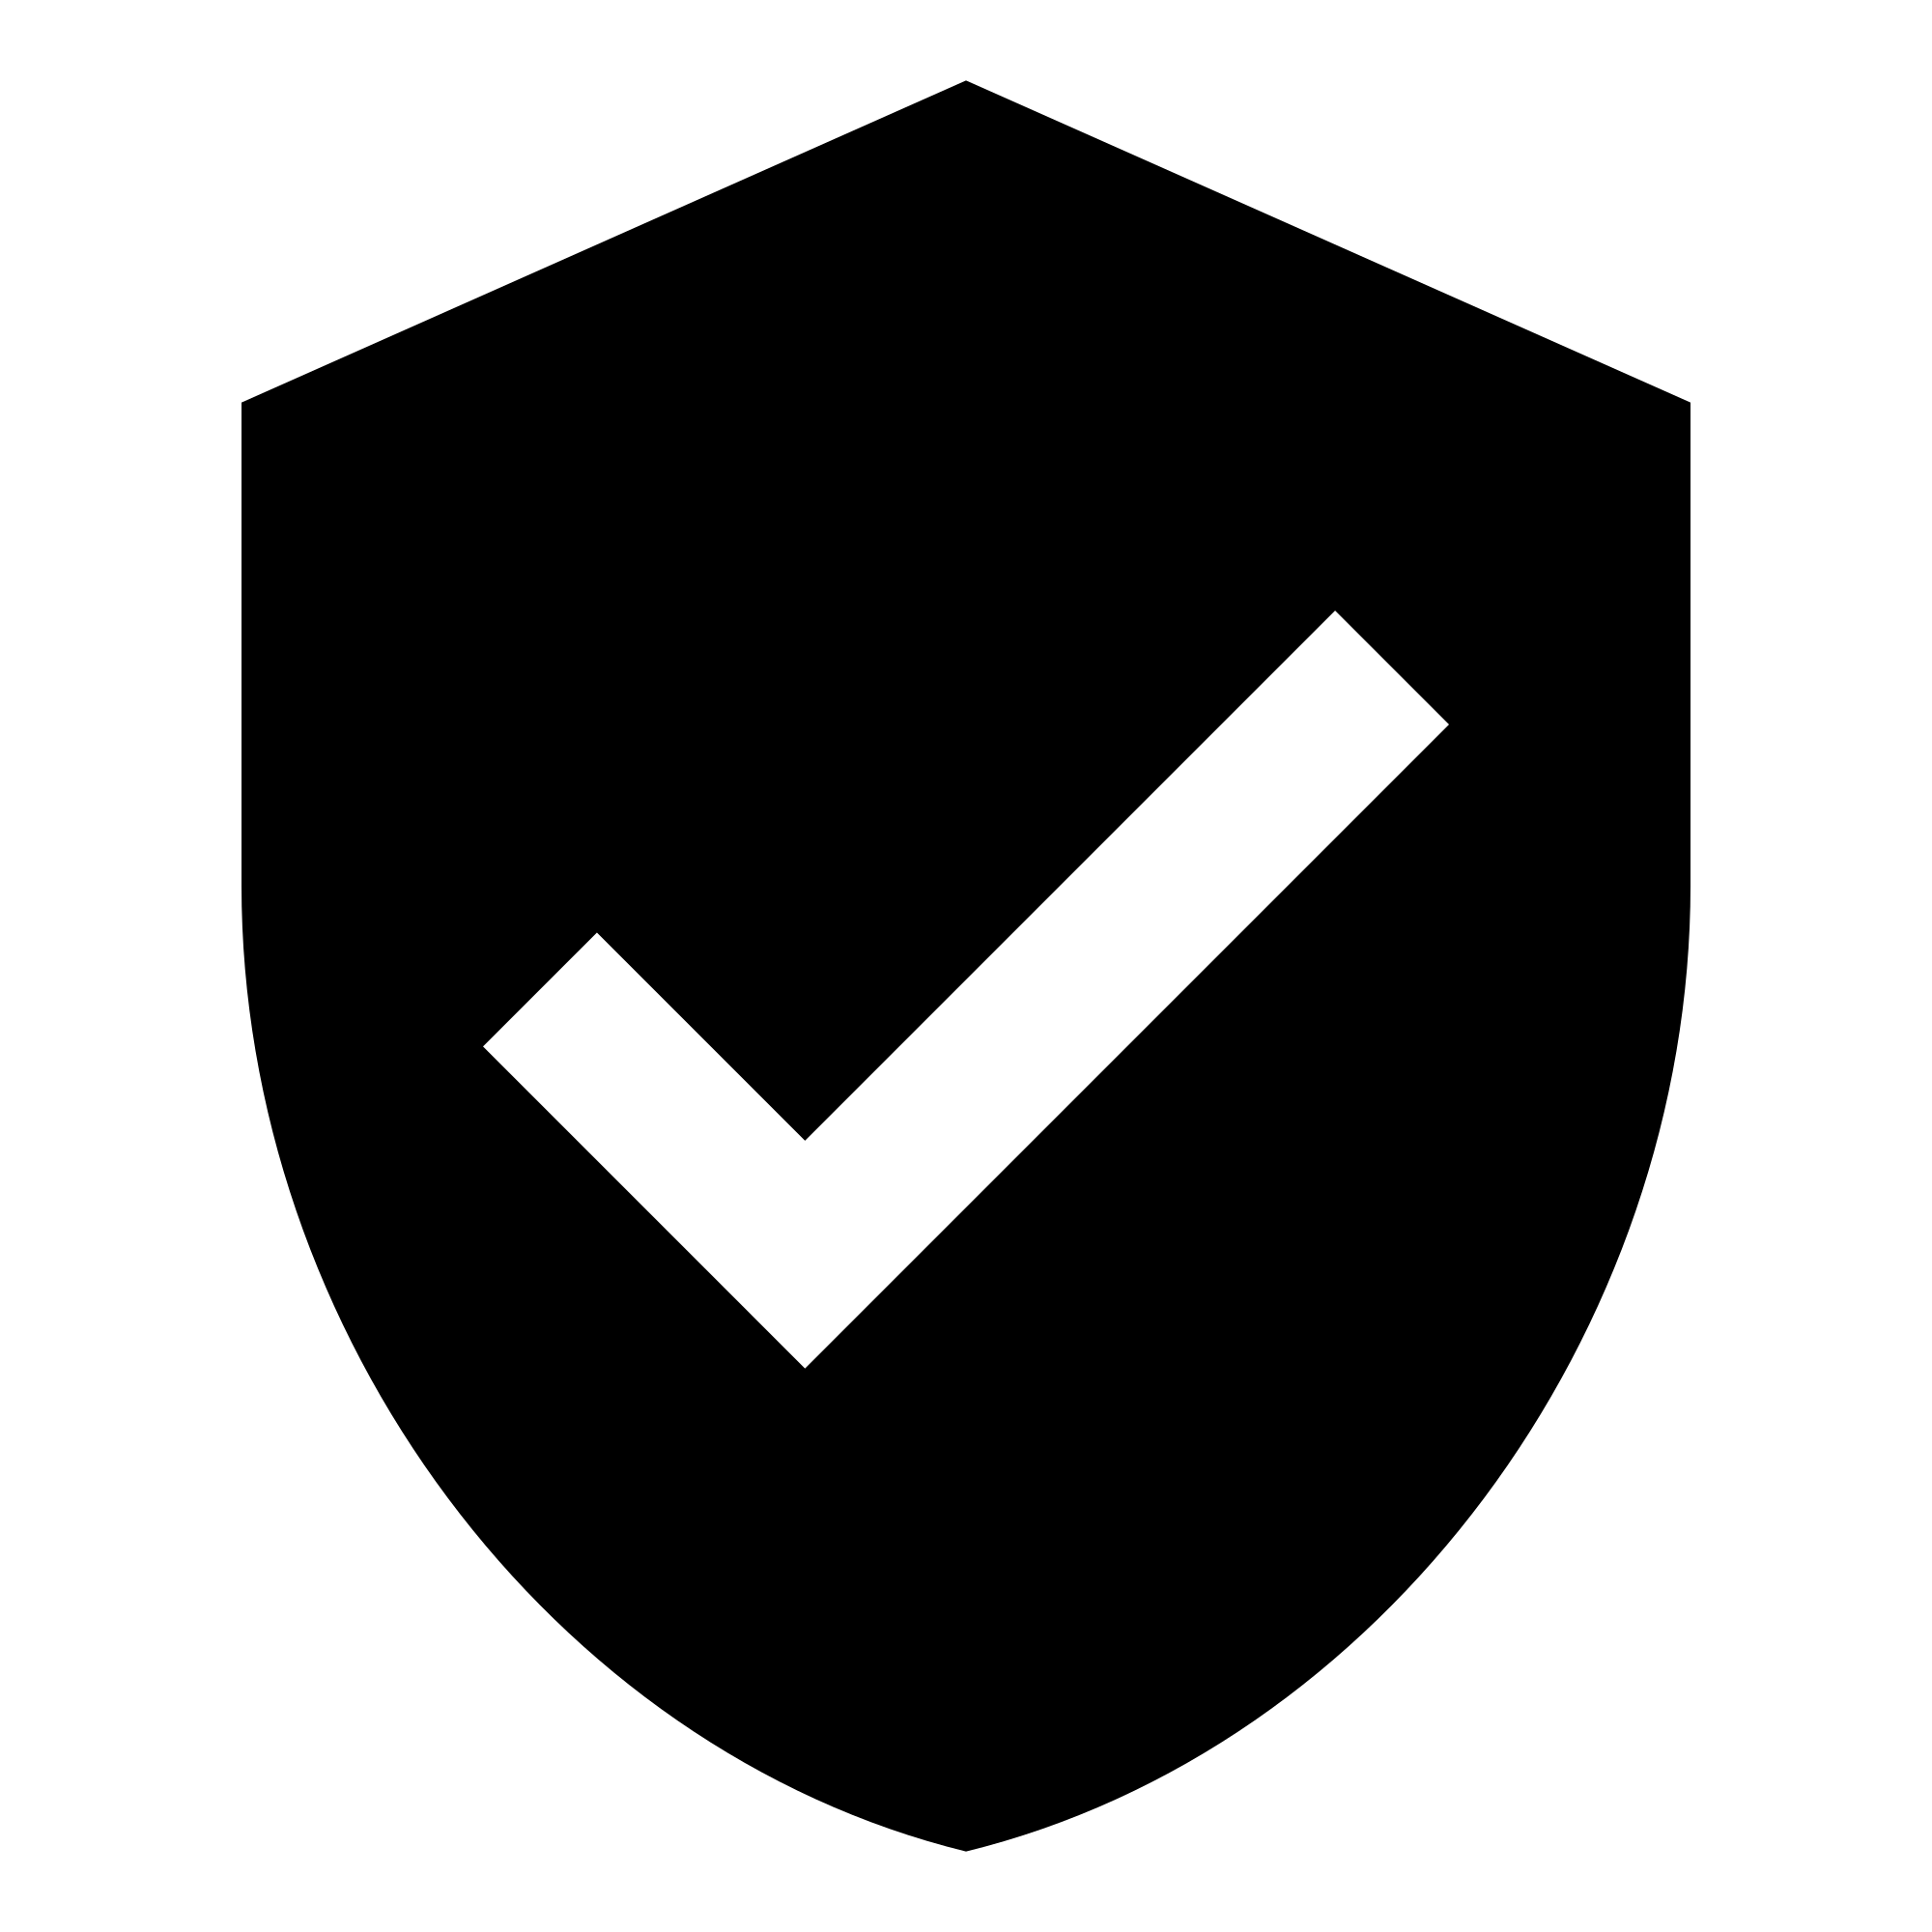
\includegraphics[scale=0.015, right]{snark.png}
%     \vspace{-1cm}

%     (Succinct Non-interactive ARguments of Knowledge)

%     \begin{itemize}

%         \item {\bf Prover} (a.k.a. Solution Proposer) does computation off-chain to prove that auction results are feasible. 
%         \item {\bf Verifyer} snark-proof is submitted on-chain in the form of a Smart Contract
%         \item Snarks used for all State Transitions (i.e. account balance updates)
%         \begin{enumerate}
%             \item Processing Deposits
%             \item Processing Withdrawals
%             \item Auction Settlement
%         \end{enumerate}
%     \end{itemize}
% }

\section{Snark Applications}

\subsection{Rudimentary Components}

\frame{
    \frametitle{Smart Contract}
    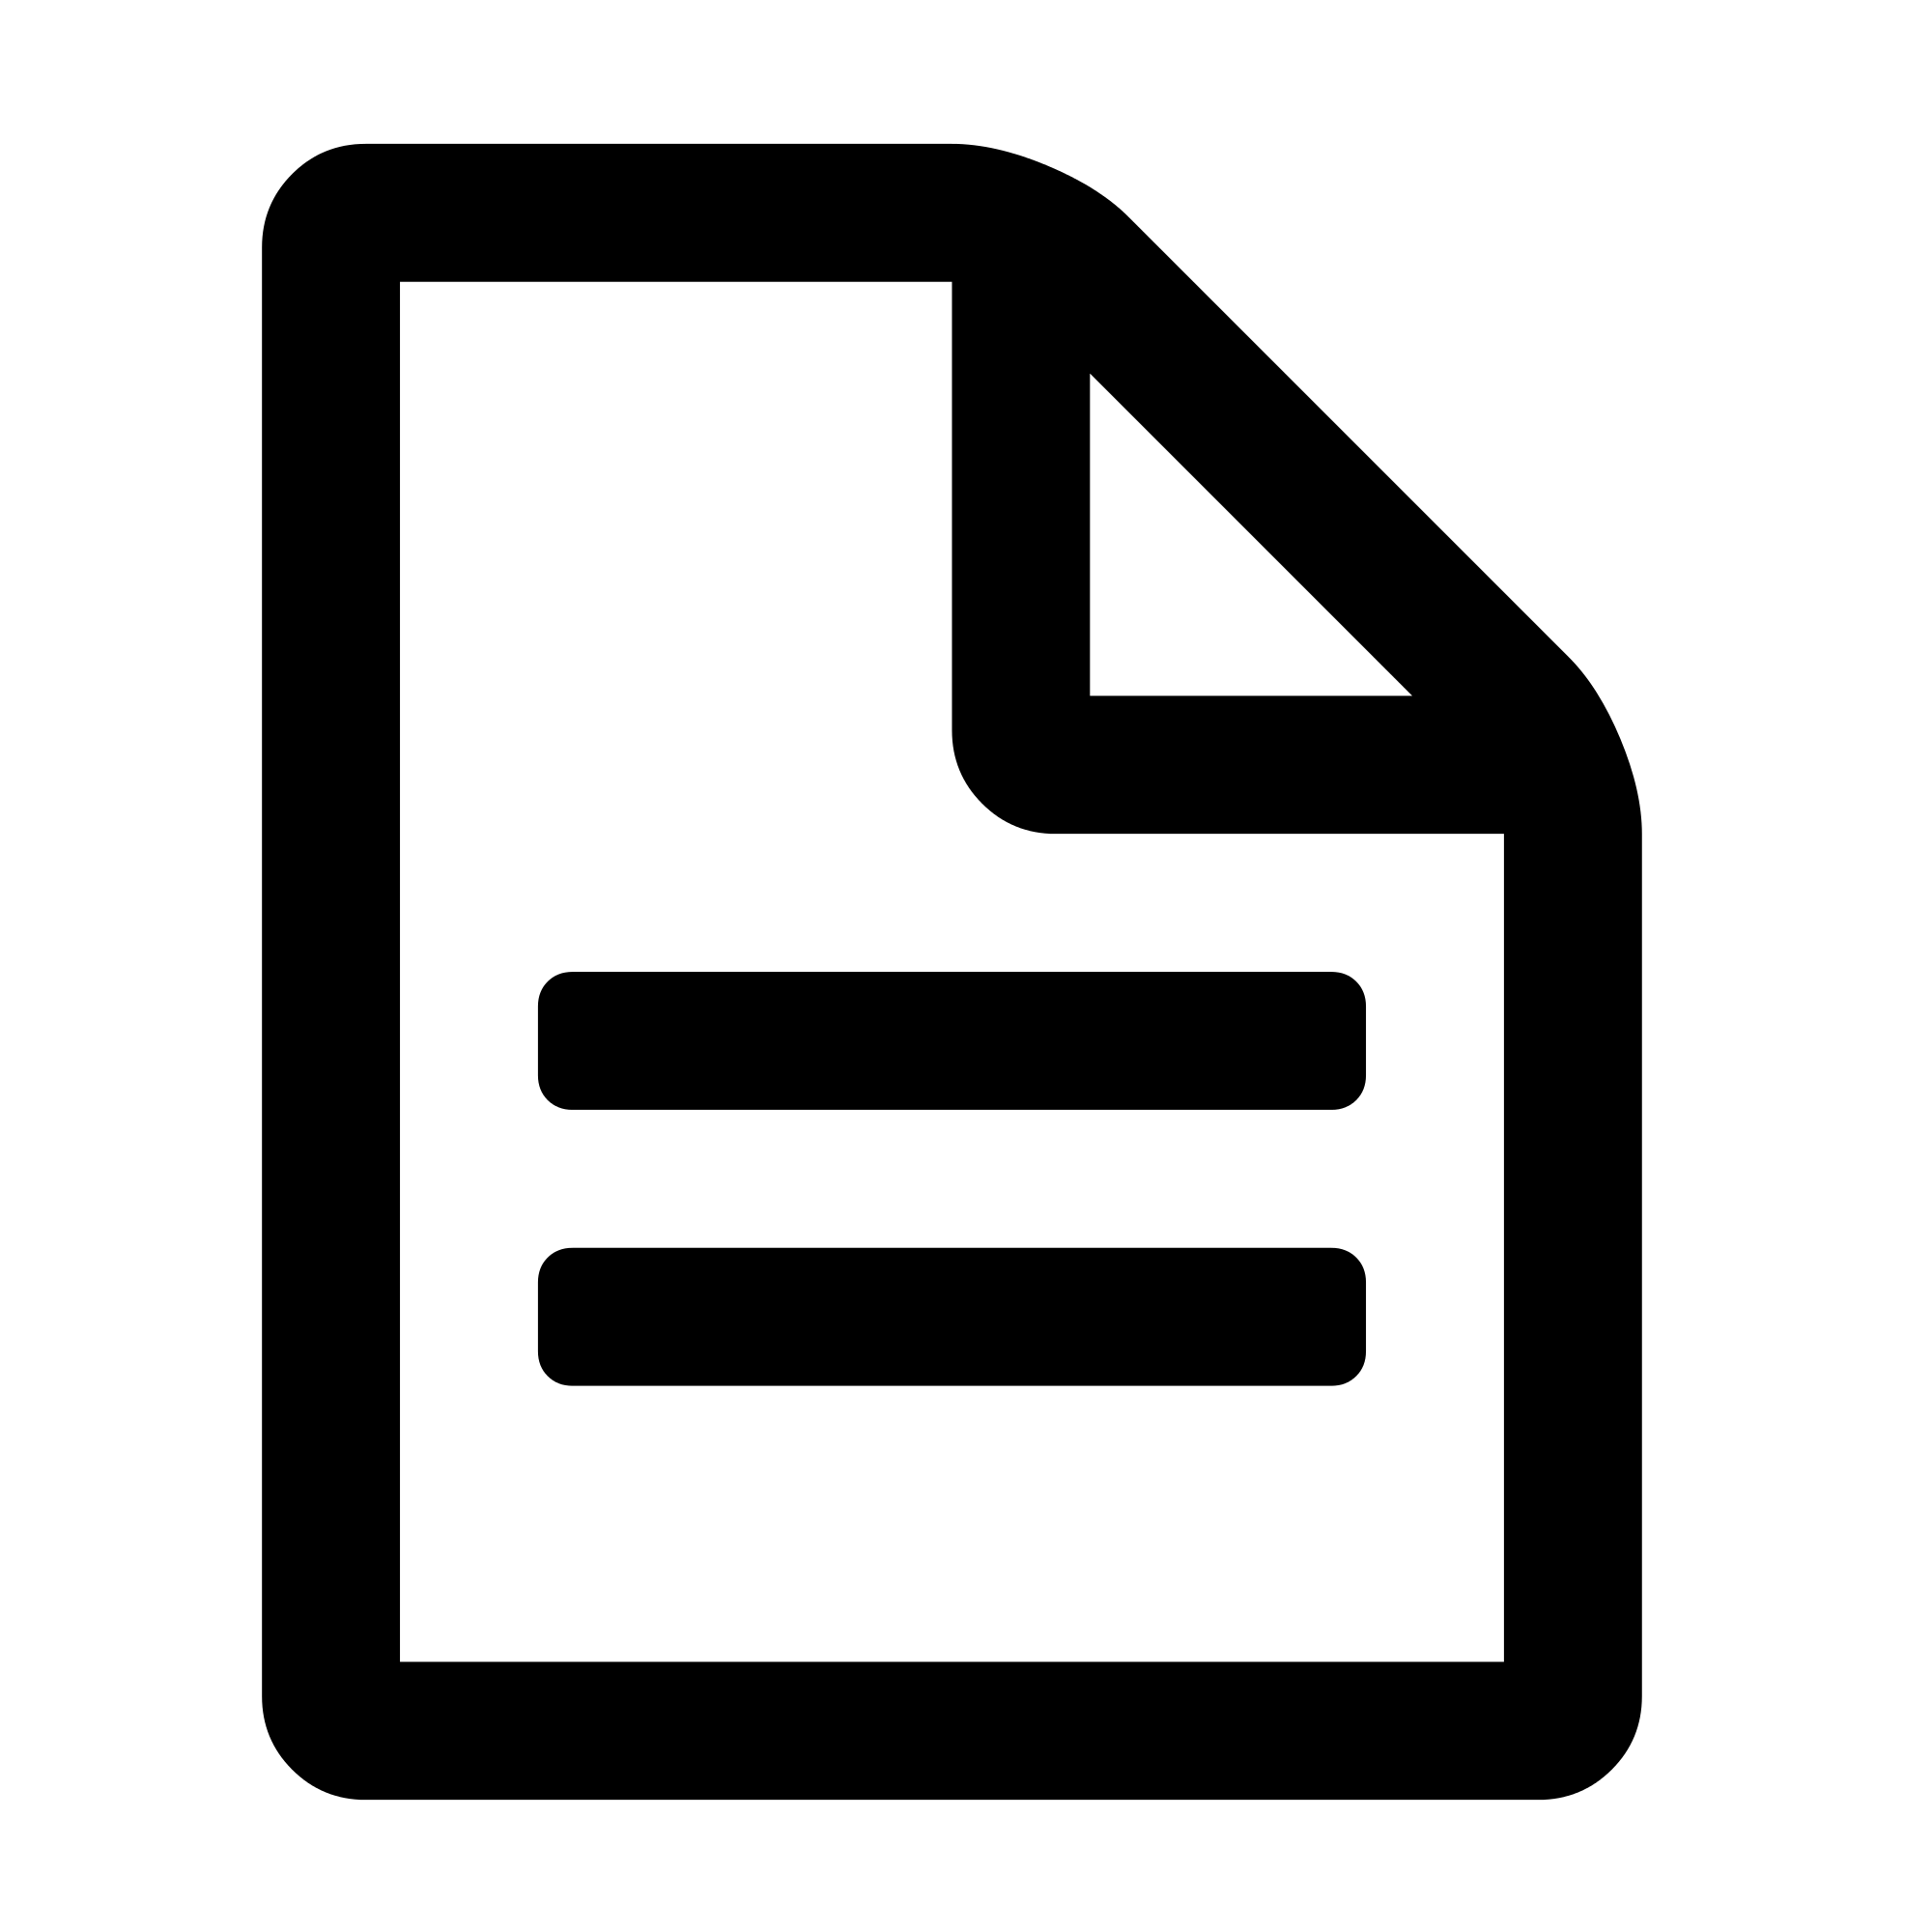
\includegraphics[scale=0.02, right]{contract.png}
    \vspace{-2cm}

    Contains
    \begin{enumerate}
        \item Elementary Items and Accessibility
        \begin{itemize}
            \item tokens, accounts and registration of them
        \end{itemize}
        \item Participation Requests
        \begin{itemize}
            \item deposit, withdraw and limit order
            \item emit events
        \end{itemize}
        \item State Transitions (balances)
        \begin{itemize}
            \item processing deposits, withdrawals and auction results
        \end{itemize}
        \item Challenge, Resolve \& Rollback
    \end{enumerate}
}

\subsection{Event Listener}

\frame{
    \frametitle{Off-chain}
    
\includegraphics[scale=0.05, right]{listener.png}
    \vspace{-2cm}
    \begin{itemize}
    \item
    Requests are emitted as an event by the Contract
    \begin{itemize}
        \item {\bf Deposit}

            "Account $k$ deposited $d$ of token $t$"
        \item {\bf Withdraw}

            "Account $k$ withdrew $d$ of token $t$"
        \item {\bf Limit Order}

            "Account $k$ to trade $\leq d$ of $t_i$ for $t_j$ if exchange rate is $\leq r$"
    \end{itemize}
    \item
    Contract doesn't store the information contained in events.
    \item
    Event Listener collecting and storing relevant info (Anyone)
\end{itemize}
}




\subsection{Contract Driver}

\frame{
    \frametitle{Off-chain}
    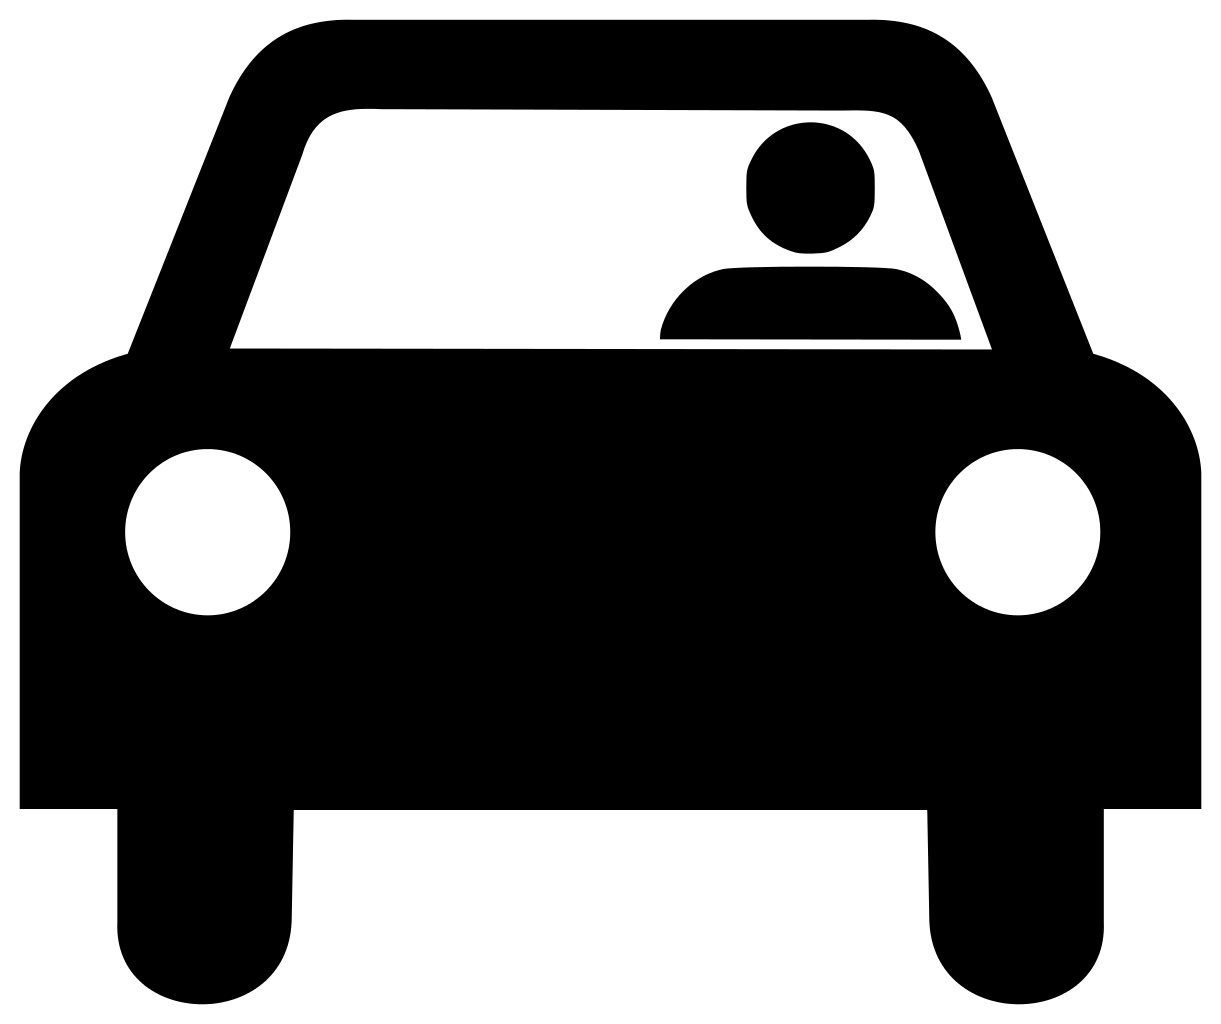
\includegraphics[scale=0.03, right]{driver.png}
    

    Information stored by listener is used to "Drive" the contract %(i.e. update Account states)

    \begin{itemize}
        \item Perform all the balance updates and hashing
        \item Call process-request functions (AccountStateTransitions)
        \item (On Challenge) Computes snark proofs
    \end{itemize}
}

% \subsection{Snarks revisited}

% \frame{
%     \frametitle{deposits \& withdrawals}
%     Snark contains all information regarding deposits in that slot
% }

% \frame{
%     \frametitle{Auction Settlement}
%     Snark contains, prices and limit-order fulfilment is sufficient to demonstrate constraints of Linear Program
% }


\section{Upcoming Challenges}

\frame{
    \frametitle{Future Features}
    \begin{enumerate}
        \item Fork-able States
        \item Basket Orders
        \item Batch Requests (i.e. offchain order collection - as a service)
        \item Continuation Orders
    \end{enumerate}
}


\frame{
    \frametitle{Resources}
    All our efforts are open-sourced through Gnosis GmbH at

    \begin{center}
        \href{http://github.com/gnosis/}{http://github.com/gnosis/}
    \end{center}

    \begin{thebibliography}{99}
        \bibitem{dFResearch} \emph{Formal Specification}: gnosis/dex-research
        \bibitem{dFContracts} \emph{Smart Contracts}: gnosis/dex-contracts
        \bibitem{dFServices} \emph{Infastructure (Listener \& Driver)}: gnosis/dex-services
    \end{thebibliography}



}


\end{document}
